\documentclass[atmp]{ipart_v1}

\usepackage{bm}
\usepackage{graphicx}
\usepackage{caption}

\def\rmd{\mathrm{d}}
\def\rme{\mathrm{e}}
\def\rmi{\mathrm{i}}

\def\S{\widehat{S}}
\def\W{\widehat{W}}
\def\C{\widehat{C}}
\def\f{\hat{f}}
\def\g{\hat{g}}
\def\h{\hat{h}}
\def\psii{\bm\psi}
\def\LL{\widehat{L}}
\def\lmbd{\bm{\lambda}}
\def\Tp{\mathrm{T}}
\def\unity{1}
\def\Re{\mathrm{Re}}
\def\Im{\mathrm{Im}}
\def\w{\omega}

\newcommand\eref[1]{\eqref{#1}}
\newcommand\Eref[1]{Equation \ref{#1}}
\newcommand\fref[1]{figure \ref{#1}}
\newcommand\sref[1]{section \ref{#1}}

\newcommand\phsintgrnd[1][z]{q(#1,\lmbd)}
\newcommand\predexp[1][z]{q(#1,\lmbd)^{-1/2}}
\newcommand\phsintgrl[3][z]{\int_{#2}^{#3} \phsintgrnd[#1] \rmd #1}

\begin{document}
\title[Symmetry relations for effective Stokes constants]{Effective Stokes diagram, symmetry relations and functional equations for effective Stokes constants}
\author[A.G. Kutlin]{A.G. Kutlin}

\begin{abstract}
We consider an arbitrary ordinary linear differential equation of the second order and study 
how its symmetries affect the Stokes constants associated with its general solution. 
We reformulate the well-known Heading's rules for analytical continuation in a matrix form 
and propose a concept of an effective Stokes diagram. We show that effective Stokes 
domains which can be overlaid by a symmetry transformation are associated with the same 
effective Stokes constant and can be described by the same analytical function. Basing on
the derived symmetry relations we propose a way to write functional equations for 
the effective Stokes constants. This work also contains an example of usage 
of the presented ideas in a case of a real physical problem.
\end{abstract}

\maketitle

\section{Introduction \label{sec:intro}}
Consider an arbitrary ordinary linear differential equation written in the form of 
a stationary one-dimensional Schr\"odinger equation:
\begin{equation}
\LL(z,\lmbd)y(z,\lmbd)=0, \quad \LL(z,\lmbd)=\frac{\rmd^2}{\rmd z^2} + Q(z,\lmbd),   \label{eq:gen}
\end{equation}
where $\lmbd$ is a set of the problem`s parameters. Throughout the paper 
$Q(z,\lmbd)$ will be referred to as a potential. It is often natural to describe two 
linearly independent solutions of \eref{eq:gen} using so-called phase-integral 
approximation. In the notation of Fr\"omans \cite{frbook}, it can be written as
\begin{equation}
y_\pm = \predexp \exp [\pm \rmi \w(z)], \quad \w(z)=\phsintgrl[\xi]{(z_0)}{z},   \label{eq:phsint}
\end{equation}
where the explicit form of $q(z)$ depends on the particular type of the approximation.
The simplest and the best-known type is one of the WKBJ\cite{wkb1,wkb2,wkb3,wkbj}; 
it takes the form \eref{eq:phsint} with $\phsintgrnd = \sqrt{Q(z,\lmbd)}$.

The function $\w(z)$ is the phase integral, and therefore we call $\phsintgrnd[\xi]$ 
the phase integrand. Also we will refer to $z_0$ as a basepoint. A meaning of the brackets in the 
lower limit of integration is a bit tricky; such a notation was introduced by Fr\"omans \cite{frpaper} to make
phase integral look similar for all orders of approximation. In the lowest order and, particularly,
in case of the WKBJ approximation, this integral is just a usual integral from $z_0$ to $z$.
 
Provided that 
\begin{equation}
\varepsilon = q^{-3/2} \rmd^2 q^{-1/2}/\rmd z^2  + (Q - q^2)/q \ll 1,   \label{eq:cond}
\end{equation}
a general solution of \eref{eq:gen} can be approximated by
\begin{equation}
y = c_+y_+ + c_-y_-. \label{eq:gensol}
\end{equation}
Clearly, the inequality \eref{eq:cond} is not valid in a vicinity of poles or zeros of 
the phase integrand. Such points will be referred to as singular points and the 
vicinity of a singularity will be referred to as the interaction area.

Any phase-integral type solution \eref{eq:phsint} is a local, not global, solution of \eref{eq:gen}. 
The method of phase integrals allows the construction of a globally defined 
asymptotic expression for the solution of a desired linear ordinary differential 
equation. The method was first proposed by A.Zwaan in his dissertation in 1929 \cite{zwaan}. 
He suggested allowing the independent variable in the differential equation to take 
complex values and to study a behaviour of the asymptotic solution far away from any 
singularities. According to Stokes\cite{stokes}, for any given exact solution 
of \eref{eq:gen} coefficients $c_+$ and $c_-$ in the approximate solution \eref{eq:gensol} 
differ from one domain of the complex plane to another 
(Stokes phenomenon \cite{stokes,white,heading,frbook}). Such abrupt 
changes happen on the so-called Stokes lines and have a form of a single-parameter 
linear transform\cite{heading}. The parameter associated with a particular Stokes line 
is called the Stokes constant. Knowing all Stokes constants associated with a particular 
potential gives the ability to obtain a globally defined approximate solution 
of \eref{eq:gen}\cite{heading,white} and the phase-integral method provides a simple 
way to find these constants and to write the solution. Unfortunately, there are very few 
cases when this method allows finding all the constants exactly, so approximations of different 
kinds are commonly used \cite{white,ours}. This happens mostly because of a lack of 
exact equations for the Stokes constants.
 
The phase-integral approximation has an extensive application in quantum mechanics and other branches of
physics, along with many attempts to improve its accuracy\cite{ours,dunham,dingle73,berry90,berry91,sergeenko96,delabaere97,sergeenko02,mirnov10,poor16,esposito09,aleixo00}. 
In the present paper we provide a recipe to reduce the number 
of independent Stokes constants for a particular problem using symmetries of \eref{eq:gen}. 

The paper is organized as follows. 
In \sref{sec:mtrxfrm} the matrix formulation of Heading`s rules is given. Such formulation appears
to be much more convenient for our purposes then the traditional one, which can be found, 
for example, in \cite{white}.
In \sref{sec:effsd} a concept of an effective Stokes diagram is presented. This concept is a natural
consequence of the matrix formulation. The idea of an effective Stokes constant is
essential for all following discussion on the subject of symmetry relations.
In \sref{sec:smmtrs} the symmetry relations are obtained from simple considerations. 
In \sref{sec:weber} the relations are used to find the exact form of reflection and 
transmission coefficients for the Weber equation. 
And, finally, in \sref{sec:cnclsns} are the conclusions. 

\section{Matrix formulation of the Heading`s rules of analytical continuation \label{sec:mtrxfrm}}
Let's start with some basic definitions. At every point $z$ of the complex plane except the 
singularities we will distinguish two orthogonal directions. Let's define the Stokes direction 
as a direction with $\Re \left[ \phsintgrnd \rmd z \right]=0$ and the anti-Stokes direction 
as a direction with $\Im \left[ \phsintgrnd \rmd z \right]=0$. We will also use a notion of 
the Stokes (anti-Stokes) field as a set of Stokes (anti-Stokes) directions for the entire 
complex plane. Following \cite{heading, white}, we introduce Stokes (anti-Stokes) lines as a 
paths along Stokes (anti-Stokes) field emanating from the potential`s singularities. 
Any domain of the complex plane bounded by the Stokes (anti-Stokes) lines and containing no other 
Stokes (anti-Stokes) lines will be referred to as the anti-Stokes (Stokes) domain. Particularly, if 
the potential $Q(z,\lmbd) \sim z^n$ as $z$ goes to complex infinity, then there are $n+2$ Stokes 
(anti-Stokes) domains in the vicinity of the infinity - we will call such domains the Stokes 
(anti-Stokes) wedges. Asymptotic phase-integral solutions \eref{eq:phsint} oscillate along anti-Stokes 
lines with constant flow and increase (or decrease) exponentially with constant phase along Stokes lines. 
The increasing (decreasing) solution will be called dominant (subdominant) in a given Stokes domain. 
Strictly speaking, for every point except points of anti-Stokes lines the subdominant solution 
should be omitted since otherwise this results in over precision, but we will keep both functions 
everywhere according to the tradition. For the same reason we will assume, that the Stokes phenomenon 
occurs strictly on the Stokes line, although it can be detected only by comparing the asymptotic forms 
of the exact solution on the neighbouring anti-Stokes lines. Also, the complex plane with singular points
of the phase integrand, Stokes and anti-Stokes lines and branch cuts associated with a 
branching structure of asymptotic solutions \eref{eq:phsint} will be referred to as a Stokes diagram.

Usually, for any solution`s analytical continuation around the interaction area 
the Heading`s rules are used. These rules determine how the coefficients $c_\pm$ 
from \eref{eq:gensol} change from one anti-Stokes domain to another. A traditional presentation 
of these rules can be found in \cite{heading, white}. For us it is convenient to transform 
these rules into the matrix form for ease of reference.

Let's define a two-dimensional vector space consisting of vectors
\begin{equation}
\psii= \left(\begin{array}{*{2}{c}} c_+ \\ c_- \end{array}\right).
\end{equation}
Then assume that we have two neighbouring anti-Stokes domains $1$ and $2$, and there are 
corresponding $\psii$-vectors in the domains. Assume also that $y_+$ is dominant in the Stokes 
domain containing a borderline separating these anti-Stokes domains. 
In this situation we can relate $\psii_1$ and $\psii_2$ through the Stokes 
operator $\S$ in the following way:
\begin{equation}
\psii_2 = \S[\pm s] \psii_1, \quad 
\S[\pm s] = \left(\begin{array}{*{2}{c}} 1 & 0 \\ \pm s & 1 \end{array}\right),    
\end{equation}
where $s$ is a Stokes constant. The sign of the Stokes constant as well as its value 
depends on the chosen base of approximate solutions $y_\pm$ and particularly on the 
basepoint $z_0$. We will use a plus sign if we cross the Stokes line in a counterclockwise 
direction relatively to the basepoint and a minus sign otherwise. If the borderline lies in 
a Stokes domain where $y_+$ is subdominant, we must use $\S^{\Tp}$ instead of $\S$, where 'T' 
denotes the transpose operation.

Obviously, $\psii$-vector in a given anti-Stokes domain depends on the chosen basepoint too. 
As it follows from \eref{eq:phsint}, a change of the basepoint from $z_0=a$ to $z_0=b$ in 
terms of $\psii$-vectors can be written as
\begin{equation}
\psii^{(b)} = \W[b,a] \psii^{(a)}, \quad 
\W[b,a] =  
\left(\begin{array}{*{2}{c}}
\rme^{\rmi \phsintgrl{(a)}{(b)}} & 0 \\ 0 & \rme^{-\rmi \phsintgrl{(a)}{(b)}} 
\end{array}\right).
\end{equation}
This is analogous to the reconnection formula in the traditional Heading`s form of the continuation 
rules and we will refer to the operator as a reconnection operator.

Finally, we have to introduce a $\C$ operator associated with crossing a branch cut. The explicit form 
of the operator depends on the phase integrand $\phsintgrnd$. Here we derive it for the simplest case  
assuming $\phsintgrnd^2$ to be a single valued function. Imagine the cut emanating from the $k^{th}$ order
singularity of squared phase integrand (positive values of $k$ corresponds to zeros and negative to poles). 
Place this singularity into the origin. Then assume we want to cross the cut in the counterclockwise  
direction from domain $1$ to domain $2$. To do it, we have to change our variable 
from $z$ to $z \rme^{2\rmi\pi}$. Such a change will affect both pre-exponential 
slow $\predexp$ dependency and the phase integral in the exponent of the asymptotic 
base. Specifically, to implement these changes we have to replace $\predexp$ by $(-\rmi)^k \predexp$ 
and $\int \phsintgrnd \rmd z$ by $(-1)^k \int \phsintgrnd \rmd z$. In compact matrix form 
it can be written as
\begin{equation}
\psii_2 = \C^k \psii_1, \quad
\C =  \left(\begin{array}{*{2}{c}} 0 & -\rmi \\ -\rmi & 0 \end{array}\right).    \label{eq:C}
\end{equation}
Analogous result was obtained in \cite{frbook}. Note that branching of the asymptotic solutions has nothing to do with an actual branching  of  an exact solution.

\section{Effective Stokes diagram \label{sec:effsd}}
Imagine a Stokes domain with several Stokes lines emerging from the common basepoint.
Crossing this domain means multiple sequential applications of either $\S$ or $\S^{\Tp}$ operators. But, as we
can see by a direct calculation, Stokes operators $\S$ as well as $\S^{\Tp}$ form a multiplicative
group:
\begin{equation}
\S[s_2]\S[s_1] = \S[s_2 + s_1], \quad
\S^{\Tp}[s_2]\S^{\Tp}[s_1] = \S^{\Tp}[s_2 + s_1].
\end{equation}
It means that every such set of Stokes constants can be replaced by a single one. It also means that,
for any particular problem, we will never need to know all these Stokes constants separately---the only
thing that matters is their sum.

Now consider the reconnection operator $\W$. As it follows from the properties of the phase integral, 
these operators also form a multiplicative group:
\begin{equation}
\W[c,b]\W[b,a] = \W[c,a].
\end{equation}
And, completely analogous to the situation discussed above, every set of sequential changes of the basepoint
can be described by a single reconnection operator.

Finally, imagine a Stokes domain with multiple Stokes lines and multiple basepoints. Crossing this 
domain in terms of $\S$ and $\W$ operators looks like
\begin{equation}
\S[s_n]\W[a_n,a_{n-1}]\S[s_{n-1}]\W[a_{n-1},a_{n-2}]\ ...\ \S[s_1]\W[a_1,a_0]\S[s_0].
\end{equation}
Note that for any $s'$ there is such $s''$ that $\S[s']\W[b,a]=\W[b,a]\S[s'']$, therefore
we can change the order of $\S$ and $\W$ operators. Hence,
every such set of operators can always be replaced by a single combination $\S[s_l] \W[a_n,a_0]$ or, 
if someone prefers different ordering, $\W[a_n,a_0] \S[s_r]$. Consequently, every Stokes domain can 
be described by the \textit{effective Stokes constant} $s$ despite the number of Stokes lines it contains. 

\begin{figure}
\centering
\noindent
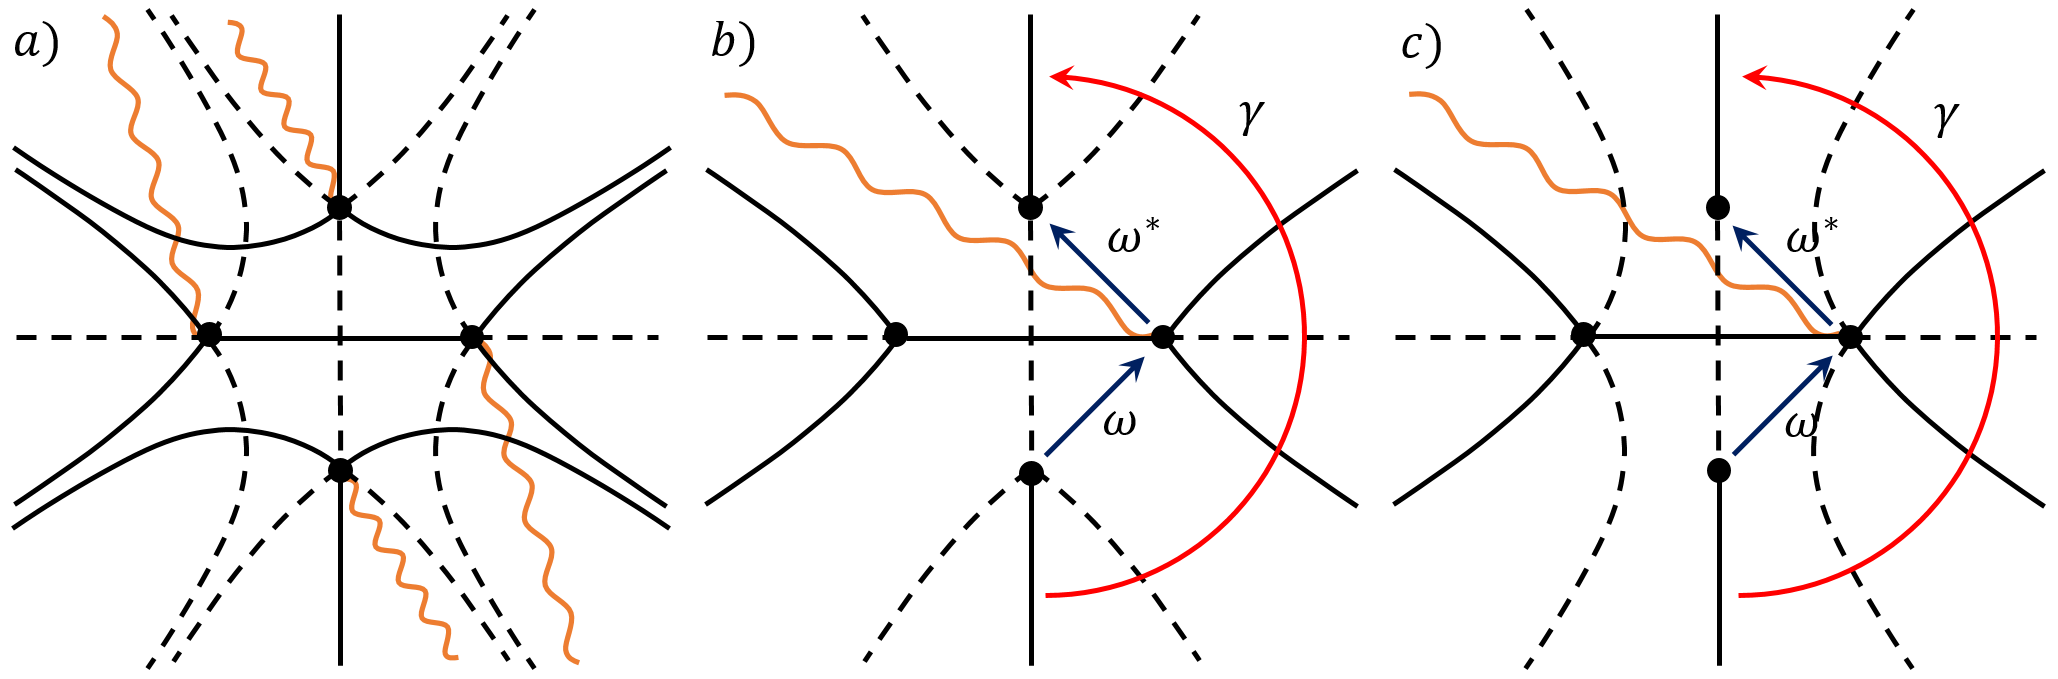
\includegraphics[width=\textwidth]{effsd_1.png}
\caption{
Stokes diagrams for $q(z,E)=\sqrt{z^4-E}$; Stokes lines are dashed
\\
(a) A traditional Stokes diagram; dots mark the zeros of the phase integrand
\\
(b) An effective Stokes diagram with a specified path of analytical continuation $\gamma$
\\
(c) An effective Stokes diagram with the same path of analytical continuation but different basepoints}
\label{fig:effsd_1}
\end{figure} 

The idea of the effective Stokes constant allows us to introduce a notion of the effective Stokes line.
Since every Stokes domain can be described by the single effective Stokes constant, we can visualize this fact 
by plotting a single effective Stokes line instead of a set of traditional Stokes lines. 
Similarly, every set of anti-Stokes lines located in the same anti-Stokes
domain can be replaced by a single effective anti-Stokes line; such a line now is just a borderline 
separating different Stokes domains. A Stokes diagram consisting of effective Stokes and anti-Stokes 
lines will be referred to as an effective Stokes diagram (figures \ref{fig:effsd_1},\ref{fig:effsd_2}). 
As it follows from the previous discussion, effective diagram is not unique
and can be plotted differently depending on the chosen path of analytical continuation (\fref{fig:effsd_2}); 
that is why it is usually convenient to specify the path right on the diagram. But even when the path is chosen we
are still free to vary our basepoints` locations. Actually, the effective Stokes line can connect any two 
points of the corresponding Stokes domain if it does not destroy the topology of the entire 
Stokes diagram, taking into account the specifics of a particular problem. 
Choosing what points to connect by the effective Stokes line we will indicate what basepoints 
will be used in the given Stokes domain (\fref{fig:effsd_1}). Also it can be useful to indicate 
values of the phase integrals instead of plotting multiple branch cuts.

\begin{figure}
\centering
\noindent
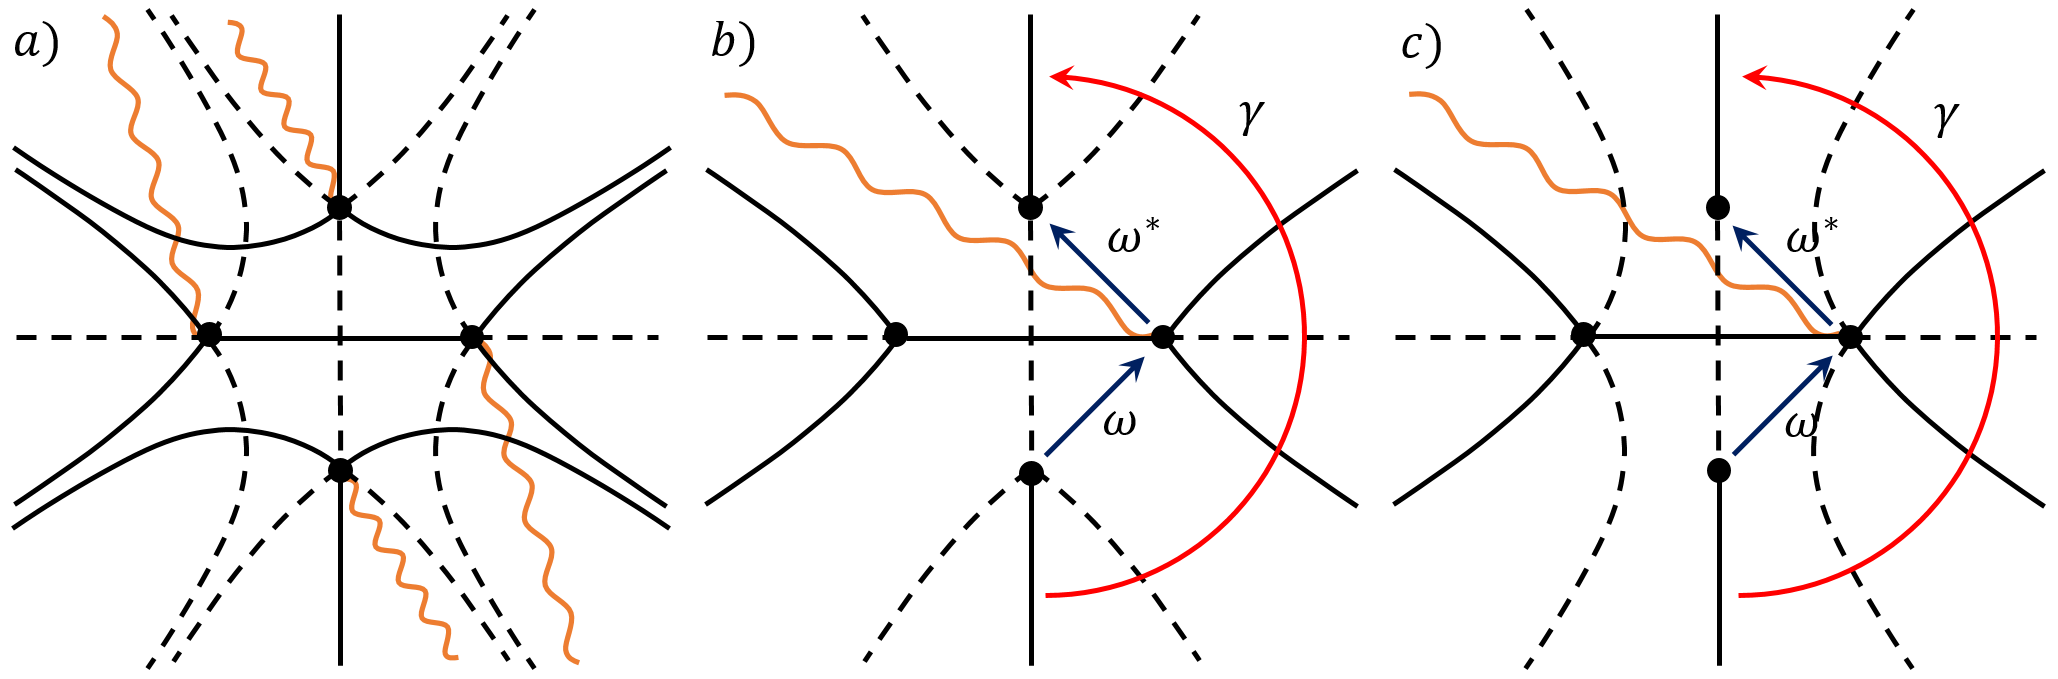
\includegraphics[width=\textwidth]{effsd_2.png}
\caption{
Stokes diagrams for $q(z,g)=\sqrt{-z + g^2/z}$; Stokes lines are dashed
\\
(a) A traditional Stokes diagram; star marks the pole of the phase integrand. 
\\
(b) An effective Stokes diagram with a specified path of analytical continuation $\gamma_1$. 
\\
(c) An effective Stokes diagram with a different path of analytical continuation $\gamma_2$.
It is meaningful only if $g \gg 1$ and all the singularities are far away from each other---otherwise 
the phase-integral approximation itself fails between the pole and the right zero and the whole theory
becomes not applicable}
\label{fig:effsd_2}
\end{figure}  

The concept of the effective Stokes constant is crucial for the following discussion. 
In contrast to the traditional one, such Stokes constant is always a computable quantity
providing the phase-integral approximation is applicable; one 
can easily calculate it by comparing asymptotics of an exact solution on the 
neighbouring anti-Stokes lines. For the traditional Stokes constant, it is present only if the
corresponding singularity is far away from any others. 
For example, let`s take a look at \fref{fig:effsd_2}. Comparing \fref{fig:effsd_2}(a) with \fref{fig:effsd_2}(b),
one can notice that the effective Stokes constant $s$ is actually a combination of
two traditional constants $s_1$ and $s_2$. If we want to calculate, for example, $s_1$, we have to continue 
some solution of the corresponding equation analytically along the path shown in  \fref{fig:effsd_2}(c). Nevertheless,
if the singularities are close to each other, the phase-integral approximation fails between the pole
and the right zero and $s_1$ loses its meaning. However, the phase-integral approximation still holds
far away from all the singularities and $s$ from \fref{fig:effsd_2} remains computable and meaningful. 

Certainly, assuming the effective Stokes constant to be analytical function of the problem`s parameters $\lmbd$
and considering that every effective Stokes constant can be expressed in terms of the traditional constants 
and corresponding phase integrals, we have to assume the traditional Stokes constant to be analytical
function as well. Under this assumptions we can analytically continue every traditional Stokes constant
from the area of the parameters` space where it is computable to the area where it is not. But even then
the only meaning of such analytically continued function is just to be a 'part' of the effective Stokes constant.
That is why any exact symmetry relation can be written only for the effective Stokes constant.

\section{Symmetries and the corresponding connections between effective Stokes constants \label{sec:smmtrs}}
Let`s define what we mean by a symmetry of a given equation. Here we introduce three operators
$\f(z,\lmbd)$, $\g(z,\lmbd)$ and $\h(z,\lmbd)$ such that
\begin{equation}
\f:\{y\} \rightarrow \{y\}, \quad
\g:\{z\} \rightarrow \{z\}, \quad
\h:\{\lmbd\} \rightarrow \{\lmbd\}.
\end{equation}
We can define any set of operators $\{\f(z,\lmbd),\g(z,\lmbd),\h(z,\lmbd)\}$ as a symmetry 
transformation of \eref{eq:gen}
if for any its solution $y(z,\lmbd)$ there is another solution $\tilde{y}(z,\lmbd)$ such that
$\tilde{y}(z,\lmbd)=\f(z,\lmbd)y(\g(z,\lmbd)z,\h(z,\lmbd)\lmbd)$, i.e.
\begin{equation}
\LL(z,\lmbd)y(z,\lmbd) \equiv 0 \ \Longrightarrow\  
\LL(z,\lmbd) \left[ \f(z,\lmbd)y(\g(z,\lmbd)z,\h(z,\lmbd)\lmbd) \right] \equiv 0.   \label{eq:symdef}
\end{equation}
For example, an Airy equation $\rmd^2 y(z)/\rmd z^2 - z y(z) = 0$ has two base symmetries: 
$\{\g=\rme^{2 \rmi \pi/3},\f=\h=\unity\}$ and $\{\f=\g=c.c.,\h=\unity\}$, where 
$c.c.$ stands 
for complex conjugation. The main difference between these two symmetries is that the second 
one changes a direction of a complex variable`s phase increase and the first one does not. 
We will refer to the symmetries of the first kind as rotation symmetries and of the second 
kind as conjugation symmetries.

The symmetry transformation`s definition \eref{eq:symdef} means that 
$\tilde{y}(z,\lmbd)$ as well as $y(z,\lmbd)$ can be written in the form \eref{eq:gensol}
but with different coefficients $c_\pm$ and $\tilde{c}_\pm$ correspondingly. 
This difference and, as a consequence, restrictions on the Stokes constants 
can be obtained directly by applying the symmetry transformation to \eref{eq:phsint}, 
but we prefer more intuitive derivation.

Every symmetry transformation can be done in three consecutive steps: transformation 
of the parameters $\h(z,\lmbd)$, transformation of the independent variable $\g(z,\lmbd)$ and 
transformation of the whole expression $\f(z,\lmbd)$. 
Certainly, both rotation and conjugation symmetries can be discrete and 
usually are, but it is much more convenient to associate some continuous transformation 
with it. This can be done by introducing of an auxiliary variable $\mu$ varying from $0$ 
to $1$ such that, for example, $\g_{cont}(\mu)=\unity+\mu (\g-\unity)$, and $\g_{cont}(1)=\g$. 
As it will be seen from the following discussion, the parametrization of the 
continuous operators can be important for the final result. Also we will assume that $\f$ can 
change the value of the effective Stokes constant but not the structure of the effective Stokes diagram and 
that is why it is not necessary to parametrize it. To determine how $\f$ acts on the 
effective Stokes constant it is enough to determine how it acts on the phase-integral approximate 
solution \eref{eq:gensol} and how it changes the coefficients $c_\pm$.

\begin{figure}
\centering
\noindent
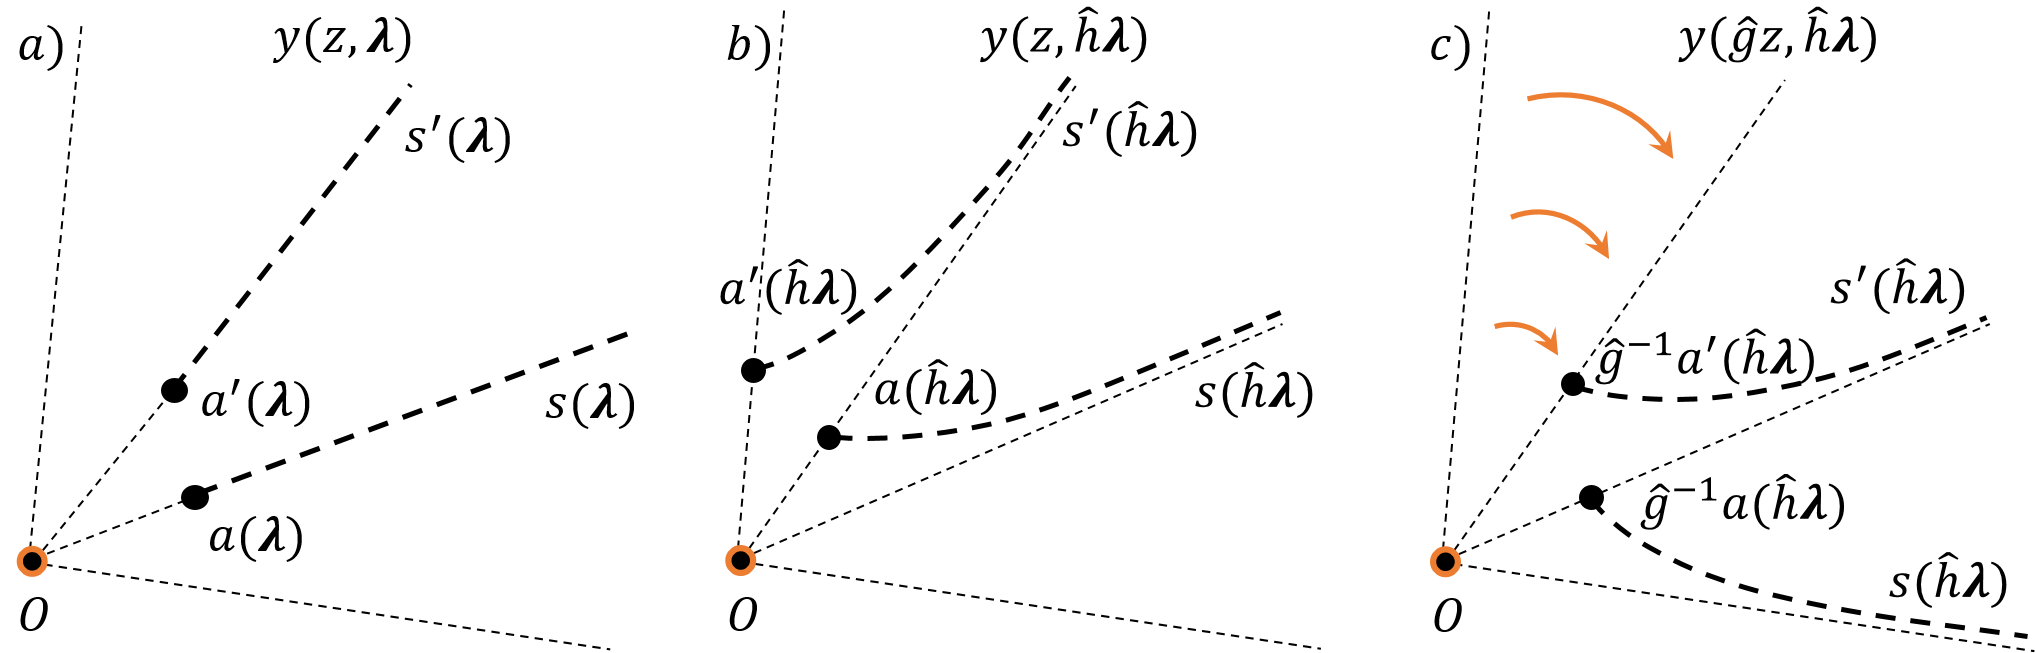
\includegraphics[width=\textwidth]{rs.png}
\caption{Effective Stokes diagram`s evolution corresponding to the symmetry transformation}
\label{fig:rst}
\end{figure}

To understand a consequences of the symmetry`s presence look at \fref{fig:rst}. 
First of all let`s keep track of the basepoints` movement under the continuous parameters` 
transformation $\h_{cont}(\mu)$. Usually it is convenient to choose some singularity of the 
potential as a basepoint, but the choice is not essential for our discussion and we will assume 
only that it somehow depends on the set of the problem`s parameters $\lmbd$. As long as under 
this assumption our basepoint $a=a(\h_{cont}(\mu)\lmbd)=a(\mu)$, like the others, is a function 
of the auxiliary variable $\mu$, the whole effective Stokes diagram continuously changes preserving its 
initial topology while $\mu$ varies from 0 to 1. Assuming also that every effective Stokes constant is 
an analytical function of $\lmbd$, we finally arrive at the situation when each transformed effective Stokes 
line associates with a new value of the same effective Stokes constant $s(\h\lmbd)$. The result of this 
transformation is shown in \fref{fig:rst}(b). 

Then, we do the same with the independent variable $z$ using $\g_{cont}(\nu)$. Under this 
transformation the Stokes domains change places and one effective Stokes line is replaced by another one 
associated with some other effective Stokes constant $s'(\h\lmbd)$ (\fref{fig:rst}(c)). Now we can see that
every symmetry relation binds such Stokes constants whose domains can be overlapped by the $\g$ 
operation. Due to the invariance of the solution space of \eref{eq:gen} 
under the symmetry transformation $\{\f(z,\lmbd),\g(z,\lmbd),\h(z,\lmbd)\}$, 
the final result of our second step can differ from the very initial 
configuration only by the basepoints` positions, and that is why $s'(\h\lmbd)$ 
and $s(\lmbd)$ have to be equal accurate to the corresponding reconnection operator
and the $\f$ transformation.

Now we are ready to write the final relation for the effective Stokes constants. A formula
expressing this relation is shown below:
\begin{equation}
\S^{(\Tp)} \left[ \f s'(\h\lmbd) \right] = 
\W \left[ \g^{-1}a'(\h\lmbd),a(\lmbd) \right]
\S^{(\Tp)} \left[ s(\lmbd) \right]
\W \left[ a(\lmbd), \g^{-1} a'(\h\lmbd) \right],
\label{eq:gensym}
\end{equation}
where $\S^{(\Tp)}$ can be either $\S$ or $\S^{\Tp}$. The choice in the right hand side 
of \eref{eq:gensym} must be made on the basis of general rules from \sref{sec:mtrxfrm}: 
we use $\S$ for the Stokes domain associated with $s(\lmbd)$ if $y_+$ is dominant 
and $\S^{\Tp}$ otherwise. In the left hand side of \eref{eq:gensym} we have to use the 
same form as in the right hand side. An integration path in the formula can be determined 
in the following way: we have to decide what path we would use to change a basepoint 
from $a(\lmbd)$ to $a'(\lmbd)$ and then trace how it deforms under our transformation. 
And now we can see why and how a resulting symmetry relation can depend on the parametrization 
of the continuous operators: this dependency is a manifestation of a branching structure of 
the effective Stokes constant as a function of the problem`s parameters $\lmbd$.

The relation discussed above must be considered as a main result of the present paper.
It allows us to take a fresh look at the nature of the different Stokes constants. 
Two different Stokes domains which can be overlapped by the transformation $\g$ are 
actually associated with the same effective Stokes constant but taken in the different 
points of the parameters` space. In particular, every set of Stokes wedges can be described 
by only one multidimensional analytical complex function $s(\lmbd)$.

Now let us take a closer look at the important special case of a complex conjugation symmetry. 
For every potential which is real on the real axes the symmetry $\f=\g=\h=c.c.$ holds, 
i.e. $\LL^*(z^*,\lmbd^*)=\LL(z,\lmbd)$ and
\begin{equation}
\S^{(\Tp)} \left[ -s'^*(\lmbd^*) \right] = 
\W \left[ a'^*(\lmbd^*),a(\lmbd) \right]
\S^{(\Tp)} \left[ s(\lmbd) \right]
\W \left[ a(\lmbd),a'^*(\lmbd^*) \right].
\label{eq:cnjgtn}
\end{equation}
A minus sign before the effective Stokes constant in the left hand side of \eref{eq:cnjgtn} is a result 
of the conjugation symmetry. It appears for any transformation $\g$ which changes the direction 
of a complex variable`s phase increase (\fref{fig:cst}). Strictly speaking, there should be two 
different general formulas for the rotation and conjugation symmetries, but it is convenient 
to agree to include this minus sign into the $\f$ operator acting on the effective Stokes constant.

\begin{figure}
\centering
\noindent
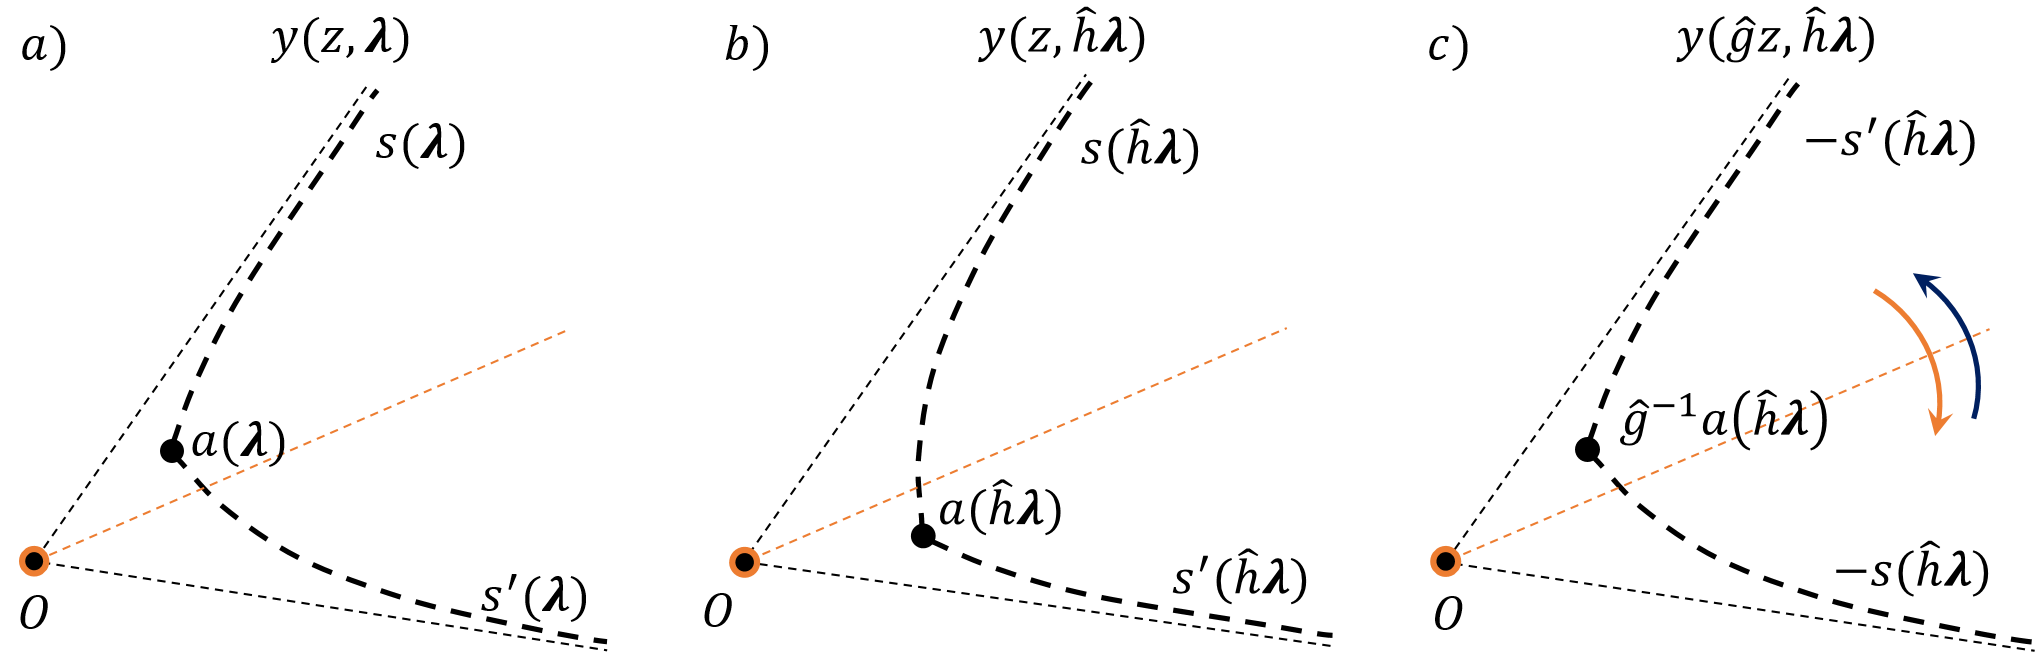
\includegraphics[width=\textwidth]{cs.png}
\caption{Effective Stokes diagram`s evolution corresponding to the conjugation 
symmetry transformation when both conjugate effective Stokes lines have the same 
basepoint and $\g^{-1}a(\h\lmbd)=a(\lmbd)$}
\label{fig:cst}
\end{figure} 

If $a(\lmbd)=a'^*(\lmbd^*)$ as in \fref{fig:cst}, and $\lmbd$ is real, we obtain a result 
$s^*(\lmbd)=-s'(\lmbd)$ which can be inferred from the symmetry relations presented in \cite{symm}. 
If furthermore $s=s'$ we get an important and extremely simple relation $s^*(\lmbd)=-s(\lmbd)$, 
i.e. such effective Stokes constant is purely imaginary providing $\lmbd$ is real.

Another important case of \eref{eq:gensym} is a case with $\g=\unity$:
\begin{equation}
\S^{(\Tp)} \left[ \f s(\h\lmbd) \right] = 
\W \left[ a(\h\lmbd),a(\lmbd) \right]
\S^{(\Tp)} \left[ s(\lmbd) \right]
\W \left[ a(\lmbd),a(\h\lmbd) \right].
\label{eq:func}
\end{equation}
Such case is relevant for every potential. The obtained relation is a functional 
equation for the considered effective Stokes constant. Usually such equation helps to illuminate 
a branching structure of the effective Stokes constant and write it as a new single-valued function 
multiplied by the known multivalued one. 
It is worth mention that even simple formal 
symmetries like $\{\h=\rme^{2\rmi\pi},\g=\f=\unity\}$
can give nontrivial functional equations; it happens always when the reconnection operator
differs from unity.

\section{Example: the Weber equation \label{sec:weber}}

\begin{figure}
\centering
\noindent
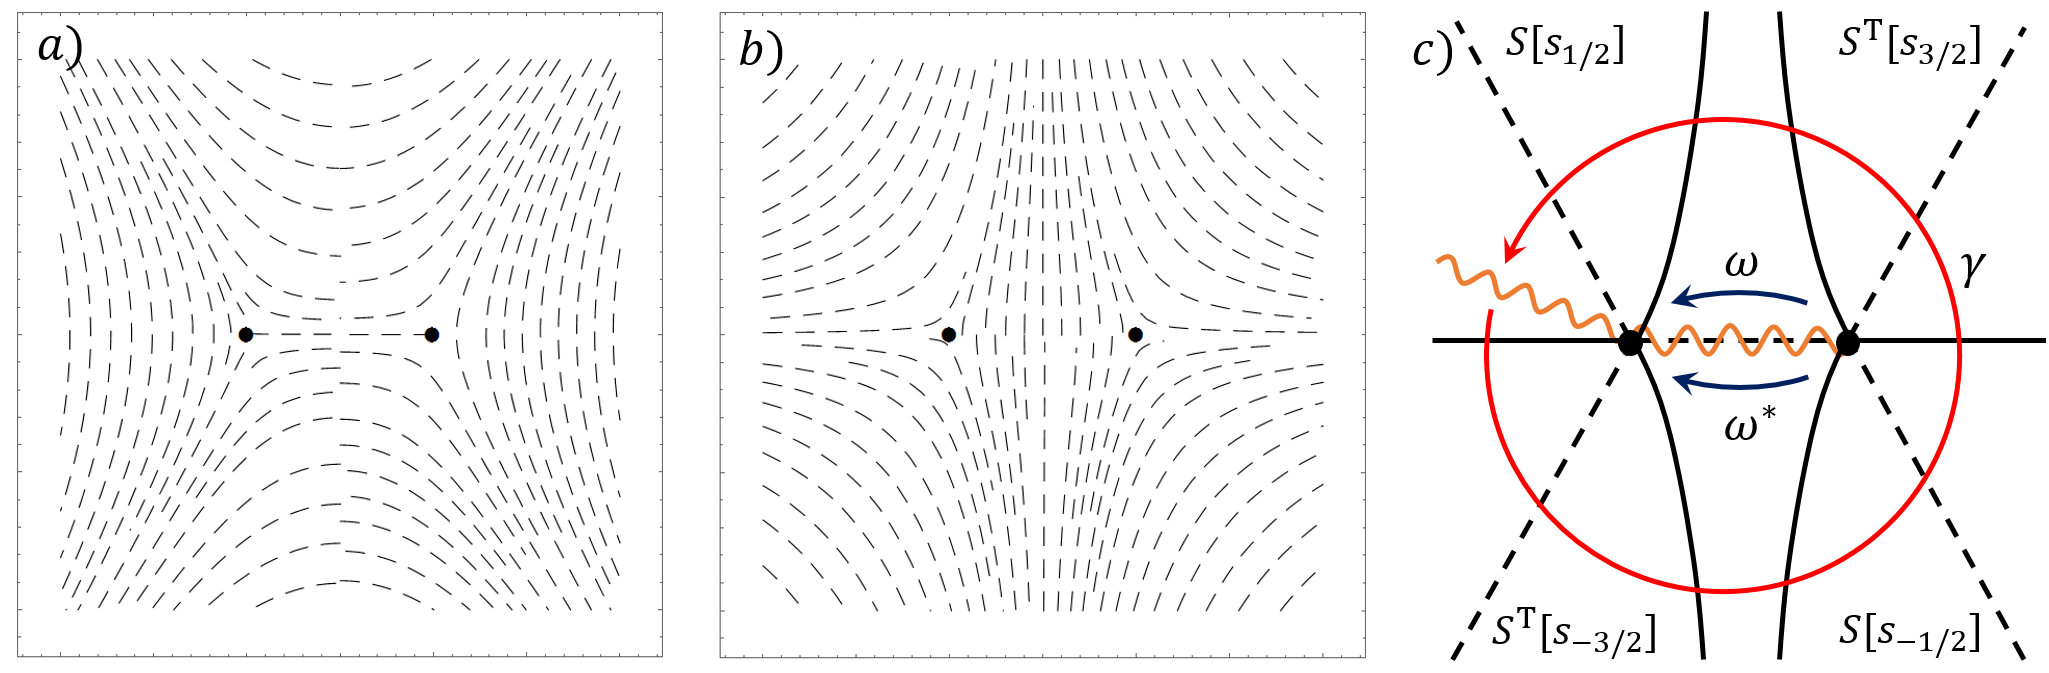
\includegraphics[width=\textwidth]{wsd.png}
\caption{Stokes field (a), anti-Stokes field (b) and an effective Stokes diagram (c) 
for the Weber equation \eref{eq:weber}}
\label{fig:wsd}
\end{figure} 

We will use WKBJ approximation all throughout this section. Also in this section we will use the symbol 
$\W[\w] \equiv \W \left[\phsintgrl{a}{b} \right] \equiv \W[b,a]$ to underline a value of the phase integral. 

Let us consider the Weber equation
\begin{equation}
\frac{\rmd^2 y(z,\delta)}{\rmd z^2}+(z^2-\delta^2)y(z,\delta)=0
\label{eq:weber}
\end{equation}
with a boundary conditions of a presence of incident wave from the large negative $z$ and absence of such 
a wave from the large positive $z$. We define the reflection (transmission) coefficient $R$ ($T$) as
a ratio of the amplitudes of the reflected (transmitted) and incident waves. 
Our aim now is to find these scattering characteristics.

The boundary conditions can be written in terms of $\psii$-vectors as
\begin{equation}
\psii_0 = \left(\begin{array}{*{2}{c}} 1 \\ 0 \end{array}\right),
\label{eq:wbound}
\end{equation}
where $\psii_0$ is a $\psii$-vector in an anti-Stokes wedge containing a ray $Arg(z)=0$.
First of all, scattering characteristics must be written through the 
Stokes constants. To do this, we must analytically continue our boundary 
condition \eref{eq:wbound} to $z$ with $Arg(z)=\pi$. 
Using \fref{fig:wsd} and the rules from \sref{sec:mtrxfrm} we write
\begin{equation}
\psii_{\pi} = 
\S \left[ s_{3/2} \right]
\W \left[ \w(\delta) \right] 
\S^{\Tp} \left[ s_{1/2} \right] \psii_0 \equiv 
\rme^{\rmi \w(\delta)} \left(\begin{array}{*{2}{c}} 1 \\ s_{3/2} \end{array}\right),
\end{equation}
where $\w(\delta)=-\rmi\pi\delta^2/2$ is a phase integral calculated above the cut 
from $z=\delta$ to $z=-\delta$. Now we have to identify incident, reflected and transmitted waves. 
Since $y_+ \propto e^{\rmi z^2/2}$ hence it is 
an outgoing wave for $z \rightarrow +\infty$ as well as for $z \rightarrow -\infty$ and
\begin{equation}
R = \frac{1}{s_{3/2}},\ T=\rmi\frac{\rme^{-\rmi w}}{s_{3/2}}.
\label{eq:RT}
\end{equation}

To find $s_{3/2}$, let`s try a traditional method described, for example, in \cite{frpaper, white}. 
We can obtain desired equations for the Stokes constants using a single-valuedness of the general 
solution and analytically continue it around the origin far away from the interaction area along the
curve $\gamma$ (\fref{fig:wsd}(c)):
\begin{equation}
\unity = 
\C^2
\S \left[ s_{3/2} \right]
\W \left[ \w \right] 
\S^{\Tp} \left[ s_{1/2} \right]
\S \left[ s_{-1/2} \right]
\W \left[ \w \right]
\S^{\Tp} \left[ s_{-3/2} \right],
\end{equation}
from which follows
\begin{equation}
\begin{cases}
s_{1/2} = s_{-3/2}\\
s_{3/2} = s_{-1/2}\\ 
s_{1/2}s_{3/2} + e^{-2 \rmi w} + 1 = 0
\label{eq:webtrad}
\end{cases}.
\end{equation}
The $\C$ operator is squared here because the Weber potential is asymptotic to $z^2$
as $z$ goes to complex infinity.

As we can see from the system \eref{eq:webtrad}, we cannot find $s_{3/2}$ using the traditional method - 
we need at least one more restriction for the Stokes constants. In \cite{white} a 
requirement of the flux conservation is used as the restriction 
and it gives $s_{-1/2}=-s_{1/2}^*$ - it helps to determine the absolute value of the
reflection coefficient, but its phase stays unknown. This example shows that even in 
a such simple situation as the Weber equation the traditional approach cannot fully 
resolve the problem.
 
Actually the flux conservation is a consequence of the real-valuedness and analyticity 
of the potential $z^2-\delta^2$ and hence the same relation can be obtained from the 
conjugation symmetry using \eref{eq:cnjgtn}. Moreover, first two equations from \eref{eq:webtrad} 
are just a consequence of a symmetry $\{\g=\rme^{\rmi\pi},\h=\f=\unity\}$---and it is clear 
because the symmetry is just a rotation and can be seen even from the usual analytical continuation. 
So, the only original equation in the system \eref{eq:webtrad} is the last one---it cannot 
be obtained from any other considerations. But these are not the only consequences of the 
equation`s symmetries, so let`s write them all.

The first nontrivial symmetry relation can be obtained from the rotation symmetry 
$\{\g=\h=\rmi,\f=\unity\}$. It can overlap, for example, Stokes domains associated with
$s_{1/2}$ and $s_{-1/2}$. Both of the Stokes constants have the same 
basepoint $a(\delta)=\delta$ and $\g^{-1}a(\h\delta)=(-\rmi)\rmi\delta=\delta$, so
\begin{equation}
\S \left[ s_{1/2}(\rmi \delta) \right] = 
\W \left[ a(\delta), a(\delta) \right]
\S \left[ s_{-1/2}(\delta) \right]
\W \left[ a(\delta), a(\delta) \right],
\end{equation}
or
\begin{equation}
s_{1/2}(\rmi \delta) = s_{-1/2}(\delta).
\label{eq:websym_1}
\end{equation}
Considering \eref{eq:webtrad}, we can 
see now that all four Stokes wedges can be described by only one function as 
was mentioned in the previous section. 

Now let's take a look at the another rotation symmetry $\{\h=\rme^{\rmi\pi},\g=\f=\unity\}$. 
As it was written in the previous section, such a symmetry gives rise to a functional 
equation which can help to illuminate a branching structure of the Stokes constant. 
For definiteness we will talk about $s_{3/2}$. To understand what to choose as endpoints 
in the phase integrals in \eref{eq:func}, let`s parametrize $\h$ as $\h_{cont}(\mu)=\rme^{\rmi\pi\mu}$ 
and look at \fref{fig:webrs}. For $s_{3/2}$ a basepoint $a(\delta)=\delta \rme^{\rmi\pi}$ 
and the question is how it is changing under our transformation. Using \fref{fig:webrs} 
we can see that finally it arrives at the point $z=\delta$, but the phase difference between the
initial and the final positions matters because it defines an integration path.
That is why we have to write $a(\h\delta)=\delta \rme^{2\rmi\pi}$ and
\begin{equation}
\S \left[ s_{3/2}(\delta \rme^{\rmi\pi}) \right] = 
\W \left[- \w \right]
\S \left[ s_{3/2} (\delta) \right]
\W \left[  \w \right],
\end{equation}
or
\begin{equation}
s_{3/2}(\delta \rme^{\rmi\pi})=s_{3/2}(\delta)\rme^{-2\rmi \w}=s_{3/2}(\delta)e^{-\pi\delta^2}.
\label{eq:websym_2}
\end{equation}
This functional equation can be solved by substitution 
$s_{3/2}(\delta)=\rmi\delta^{\rmi\delta^2}f(\delta^2)$, where $f(\delta^2)$
is single-valued in a sense $f(x)=f(x \rme^{2\rmi\pi})$.

\begin{figure}
\centering
\noindent
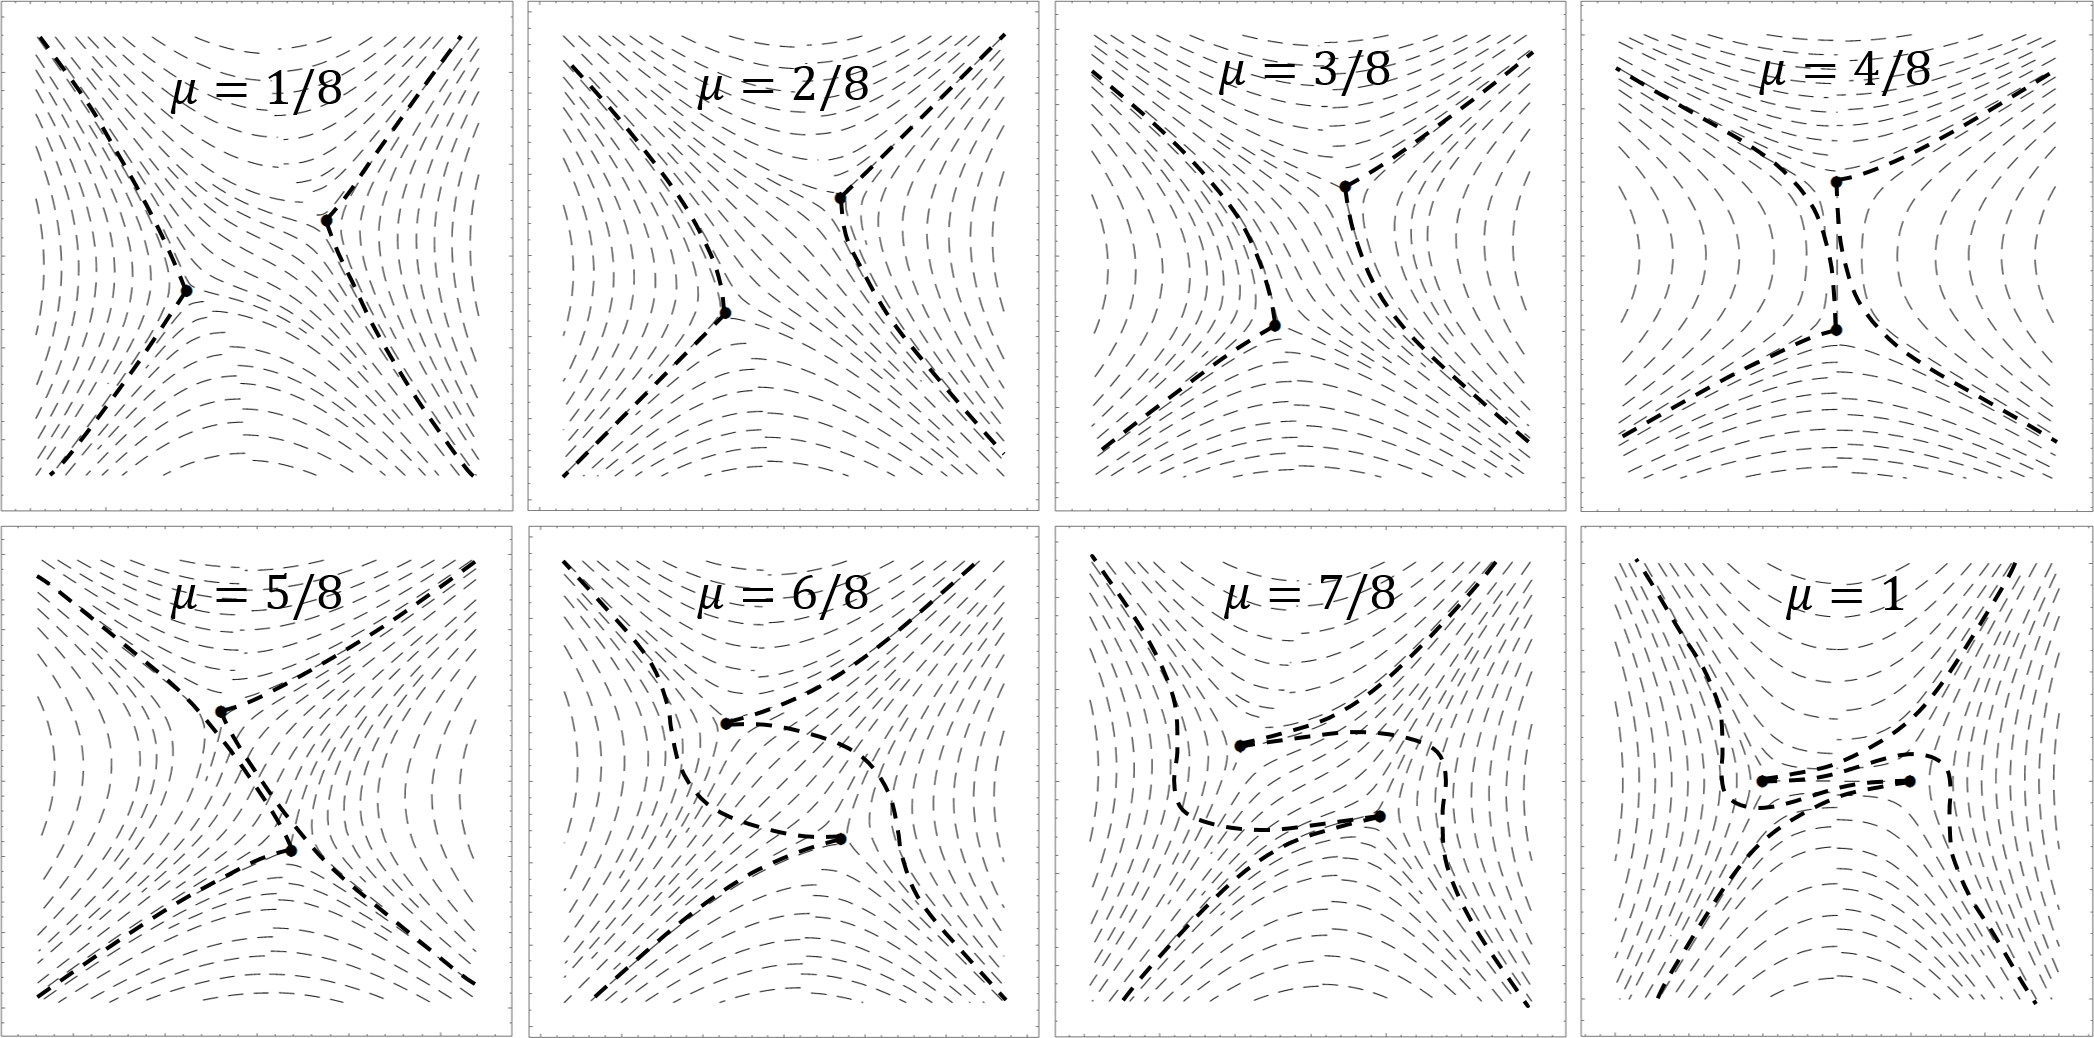
\includegraphics[width=\textwidth]{wrs.png}
\caption{Evolution of the Stokes field and effective Stokes lines 
under the continuous parameter`s transformation $\h_{cont}(\mu)=\rme^{\rmi\pi\mu}$}
\label{fig:webrs}
\end{figure} 

And, finally, consider a conjugation symmetry $\f=\g=\h=c.c.$. This symmetry relates the 
Stokes constants in the upper half of the complex plane with the constants in the lower half. 
In particular, according to \eref{eq:cnjgtn},
\begin{equation}
\S \left[ -s_{1/2}^*(\delta^*) \right] = 
\W \left[ b^*(\delta^*),a(\delta) \right]
\S \left[ s_{-1/2}(\delta) \right]
\W \left[ a(\delta),b^*(\delta^*) \right],
\end{equation}
and, since $b(\delta)=a(\delta)=\delta$,
\begin{equation}
s_{1/2}^*(\delta^*)=-s_{-1/2}(\delta).
\label{eq:websym_3}
\end{equation}
For real values of $\delta$ the last relation is nothing but the law of the flux conservation 
mentioned above. But, for complex values, together with \eref{eq:websym_2} and \eref{eq:webtrad} 
it gives
\begin{equation}
s_{3/2}(\delta)=s_{-1/2}(\delta)=\rmi(\rmi \delta^2)^{\rmi \delta^2/2}p(\rmi \delta^2),
\label{eq:websym_4}
\end{equation}
where $p(x)=p(x \rme^{2\rmi\pi})$ and $p(x)$ is real on the real axis. Now, using \eref{eq:websym_1} 
and the last equation from the system \eref{eq:webtrad}, we can write a functional equation for $p(x)$:
\begin{equation}
p(x)p(-x)=2\cos(\pi x/2).
\label{eq:pfunc}
\end{equation}
This functional equation is similar to Euler`s reflection formula \cite{gamma} and can be reduced 
to the formula by substitutions $x=1-2t$ and $p(x)=u(x)\sqrt{2\pi}/\Gamma(1/2+x/2)$, where $u(x)u(-x)=1$. 
The function $u(x)$ can be found from the boundary conditions of \eref{eq:pfunc}. Indeed, we know 
exactly \cite{white} that $s_{3/2}(0)=\rmi\sqrt{2}$. We also can assume, according to the approximation of 
isolated singularities\cite{white,ours}, that every Stokes constant approaches an imaginary 
unit as $\delta$ goes to plus infinity. Taking into consideration \eref{eq:websym_4}, we can say that
\begin{equation}
\begin{cases} 
p(0) = \sqrt{2} \\
p(x) \sim x^{-x/2}\ as\ x \rightarrow \pm \rmi \infty 
\end{cases}.  
\end{equation}
Using the asymptotics of gamma function and definition of $u(x)$, we can finally write 
that $u(x)=(2 \rme)^{-x/2}$ and
\begin{equation}
s_{3/2}(\delta)=\rmi(\rmi\delta^2)^{\rmi\delta^2/2}
\frac{\sqrt{2\pi}(2\rme)^{-\rmi\delta^2/2}}{\Gamma(1/2+\rmi\delta^2/2)}.
\label{eq:s3/2}
\end{equation}
This is an exact expression of the effective Stokes constant for 
the Weber problem---it can be verified using 
an exact solution of \eref{eq:weber} as it was done in \cite{ours}. 
Now the desired scattering characteristics \eref{eq:RT} can be found.

\section{Conclusion \label{sec:cnclsns}}

The method of phase integrals is a beautiful and powerful method of a linear ordinary 
differential equations` asymptotic analysis, but its range of applicability is highly 
restricted to relatively simple problems; more complicated problems need additional equations 
for the Stokes constants. The analysis, presented in this paper, allows the reader to find 
functional relations between different Stokes constants and thus to reduce the number of unknowns.

The main result of the present work is stated by \Eref{eq:gensym}. This result, 
like any others obtained in the paper, is valid for any approximation of the 
phase integral type, not only for WKBJ approximation. To obtain this result 
we transformed Heading`s rules \cite{heading,white} into the matrix form; 
it helped to achieve simplicity and automate the procedure of analytical continuation. 
We also proposed the idea of an effective Stokes diagram which can be a useful tool 
for simplifying the computations in case of complicated equations. 
We showed that the idea of the effective Stokes constant is crucial in context of symmetry relations;
such relations cannot be written in a general case without this idea. 
Effective Stokes constant is assumed to be analytical function with respect to 
the parameters of the problem. 
We also showed that every differential 
equation has some formal symmetries (e.g. $\{\h=\rme^{2\rmi\pi},\g=\f=\unity\}$) which may lead
to nontrivial relations for the Stokes constants. 

The functional equations which can be obtained using \Eref{eq:gensym} are likely to be as 
complex as the initial differential equation; however, they are strict and can be used as 
a basis for the construction of perturbation theory (will be a matter of a separate paper).

\section*{Acknowledgments}
This work was supported by the Russian Science Foundation (grant No~14-12-01007). 

\begin{thebibliography}{30}

\bibitem{frbook} Fr\"oman N. and Fr\"oman P.O. \textit{Physical Problems Solved by the Phase-Integral Method} (Cambridge: Cambridge University Press, 2002)

\bibitem{wkb1} G. Wentzel, Zeit. f. Phys. \textbf{38}, 518 (1926).

\bibitem{wkb2} H. A. Kramers, Zeit. f. Phys. \textbf{39}, 828 (1926).

\bibitem{wkb3} L. Brillion, C. R. Acad. Sci. Paris \textbf{183}, 24 (1926).

\bibitem{wkbj} H. Jeffries, Philos. Mag. [7] 33, 451 (1942)

\bibitem{frpaper} Fr\"oman N., Fr\"oman P.O. and Lundborg B. \textit{The Stokes constants for a cluster of transition
points} Math. Proc. Cambridge Philos. Soc. \textbf{104} (1988), 153-179.

\bibitem{zwaan} Zwaan A., \textit{Intensit\"aten im Ca-Funkenspektrum}, Academish proefschrift thesis (Utrecht, 1929)

\bibitem{stokes} Stokes, G. G., Trans. Camb. Phil. Soc. \textbf{10}, 105 (1857).

\bibitem{white} R. B. White,
 {\it Asymptotic Analysis of Differential Equations}, Imperial College Press, 2010.

\bibitem{heading} J. Heading. {\it An Introduction to Phase Integral Methods} 
Wiley, NY (1962)

\bibitem{ours} R.B. White, A.G. Kutlin, arXiv:1704.01170 (2017)

\bibitem{dunham} L. Dunham, J. Phys. Rev. X. 41. 713-720. 10.1103/PhysRev.41.713 (1932).
 
\bibitem{dingle73} R.B. Dingle {\it Asymmpotic Expansions: Their Derivation and 
Interpretation} Academic Press, London and New York (1973)

\bibitem{berry90} M.V. Berry and C.J. Howlse, Proc.Roy.Soc.Lond.,A430,653 (1990)

\bibitem{berry91} M.V. Berry, Asymmpotics, Superasymptotics,
 Hyperasymptotics, in {\it Asymptotics Beyond All Orders}, H. Segur et al (eds.) Plenum Press NY (1991)

\bibitem{sergeenko96} M.N. Sergeenko, Physical Review A. [53] 3798 (1996)

\bibitem{delabaere97} E. Delabaere, H. Dillinger, and F. Pham, J. Math. Phys. [38] 6126 (1997)

\bibitem{sergeenko02} M.N. Sergeenko, ArXiv:quant-ph/0206179v1 (2002)

\bibitem{mirnov10} A. Mirnov and A. Morozov, Journal of High Energy Physics 2010:40 (2010)

\bibitem{poor16} A.K. Kashani-Poor, ArXiv:1604.01690v3 (2016)

\bibitem{esposito09} G. Esposito and P. Santorelli J. Phys. A: Math. Theor. 42 395203 (2009)

\bibitem{aleixo00} A.N.F. Aleixo et al J. Phys. A: Math. Gen. [33] 1503 (2000)

\bibitem{symm} Fr\"oman, N., Fr\"oman, P. O., and Lundborg, B., 1988b, 
Math. Proc. Camb. Phil. Soc. \textbf{104}, 181–191

\bibitem{gamma} M. Abramowitz and I. A. Stegun, eds., 
{\it Handbook of Mathematical Functions With Formulas, Graphs, and Mathematical Tables}, 
NBS Applied Mathematics Series \textbf{55}, National Bureau of Standards, Washington, DC (1964).

\end{thebibliography}
\end{document}
